\documentclass[12pt, a4paper]{article}
\usepackage[utf8]{inputenc}
\usepackage{geometry}
\usepackage{graphicx}
\usepackage{titlesec}
\usepackage{titling}
\usepackage{array}
\usepackage{booktabs}
\usepackage{changepage}
\usepackage{fancyhdr}
\usepackage{minted} 



\geometry{left=1cm, right=1cm, top=1cm, bottom=1cm}

\title{\textbf{LAPORAN\\ Sistem dan Jaringan Komputer\\ Sistem Forwarding Pesan ke Email dan Web Server Berbasis Socket TCP }}
\author{}
\date{}
\begin{document}

\maketitle
\thispagestyle{empty}

\begin{center}
\vspace{-1.5cm}

\includegraphics[width=9cm]{Logo_PENS.png} 
\end{center}

\vspace{1cm}

\begin{center}
    \textbf{DISUSUN OLEH :}\\[0.5cm]
    KELOMPOK 9\\[0.7cm]
	\begin{tabular}{@{}l @{\hskip 2cm} r@{}}
        Muqsith Barru Pamungkas & (2423600035) \\
        Miftakhul Zannah & (2423600046) \\
        Andika Rifan Rafiudins & (2423600055) \\
    \end{tabular}
\end{center}
\vspace{0.1 cm}
\begin{center}
    \textbf{DOSEN :}\\
    Prof. Ir. Amang Sudarsono S.T., Ph.D
\end{center}

\vfill

\begin{center}
    \textbf{PROGRAM STUDI TEKNOLOGI REKAYASA INTERNET}\\
    \textbf{DEPARTEMEN TEKNIK ELEKTRO}\\
    \textbf{POLITEKNIK ELEKTRONIKA NEGERI SURABAYA}\\
    \textbf{2024/2025}
\end{center}


\newpage
\pagenumbering{arabic}
\setlength{\footskip}{10pt}
\begin{center}
    \textbf{ABSTRAK}\\[0.4cm]
\end{center}
\quad\quad Proyek ini bertujuan untuk mengembangkan dan mengimplementasikan sistem message forwarding berba-
sis protokol TCP dan teknologi Node.js untuk mendukung pengiriman
pesan melalui email serta penampilannya pada halaman web. Sistem ini dirancang dalam lingkungan
jaringan lokal (LAN) dan terdiri dari tiga komponen utama: client, forwarding server, dan email server.
Dalam alur kerjanya, client mengirimkan data berupa pesan dan alamat email yang diterima oleh forward-
ing server melalui protokol TCP. Forwarding server memproses pesan tersebut dan meneruskannya
ke dua jalur utama: server email untuk dikirimkan ke alamat tujuan melalui protokol SMTP menggu-
nakan format standar MIME, dan interface untuk menampilkan pesan secara dinamis di halaman web.
Pengujian sistem menunjukkan bahwa komunikasi antara client dan forwarding server melalui socket
TCP/UDP berjalan stabil dan efisien, dengan latensi yang rendah. Pesan yang dikirimkan berhasil
diteruskan ke server email untuk dikirimkan ke alamat tujuan, dan dapat ditampilkan secara real-time
di halaman web. Integrasi Interface memungkinkan pesan ditampilkan secara terorganisir dalam antarmuka
web yang mudah diakses. Dengan keberhasilan ini, sistem dapat berfungsi sebagai prototipe dasar untuk
kebutuhan komunikasi berbasis jaringan, baik di lingkungan akademik maupun industri, khususnya dalam
skenario pengelolaan pesan di jaringan lokal
\newline
\newline
\noindent Kata kunci: Message forwarding, TCP, Interface, Email server, Web-based messaging, komunikasi jaringan. 


\pagebreak
\titleformat{\section}{\centering\Large\bfseries}{BAB \Roman {section}}{1em}{}
\titleformat{\subsection}{\large\bfseries}{\thesubsection}{1em}{}

\section{\centering\\PENDAHULUAN}

\subsection{Latar Belakang}
\begin{adjustwidth}{1.4cm}{0cm}
\quad\quad Pemahaman tentang sistem komunikasi client-server menjadi salah satu kompetensi yang harus dikuasai dalam pembelajaran teknologi informasi. Salah satu implementasi penting dari sistem ini adalah bagaimana mengintegrasikan berbagai layanan seperti email server dan web server untuk mendukung pengiriman dan penampilan pesan secara terstruktur dan efisien. Untuk mencapai hal tersebut, diperlukan pemahaman mendalam mengenai protokol komunikasi seperti TCP/UDP yang digunakan untuk menjalin koneksi antara client dan server, serta mekanisme forwarder server yang berfungsi sebagai perantara dalam pengiriman pesan ke layanan tujuan.

Dalam konteks ini, pengiriman pesan ke email server melalui protokol email client-server menjadi salah satu metode utama untuk mendistribusikan informasi langsung ke penerima. Di sisi lain, penggunaan Interface memungkinkan web server menampilkan data secara dinamis, sehingga pesan yang diterima dari client dapat diakses dan dilihat. Tugas ini bertujuan untuk memberikan pemahaman mendalam tentang cara kerja komponen-komponen tersebut dan bagaimana mengintegrasikannya dalam sebuah sistem yang andal.

Melalui tugas ini, diharapkan mahasiswa mampu mengaplikasikan teori yang telah dipelajari ke dalam praktik, serta memiliki kemampuan analisis untuk merancang sistem yang efisien dan sesuai kebutuhan. Hal ini tidak hanya bermanfaat dalam konteks akademik, tetapi juga sebagai persiapan menghadapi tantangan dunia kerja di bidang teknologi informasi dan komunikasi.
\end{adjustwidth}

\subsection{Masalah}
\setlength{\leftmargini}{1.75cm}
\begin{enumerate}
\item Bagaimana cara membangun sistem pengiriman pesan antara client dan server forwarder menggunakan komunikasi socket TCP?
\item Bagaimana cara memforward pesan dari client melalui forwarder server ke email server menggunakan pengiriman email melalui protokol SMTP?
\item Bagaimana cara memforward pesan dari client ke web server dan menampilkan pesan tersebut di halaman interfacae web?
\end{enumerate}

\subsection{Solusi dan Rencana Realisasi Solusi}
\begin{adjustwidth}{1.4cm}{0cm}
\quad Untuk membangun sistem pengiriman pesan antara client dan server forwarder menggunakan komunikasi socket TCP, langkah pertama adalah membuat server socket di sisi server yang dapat menerima koneksi dari client. Server ini akan mendengarkan pada port tertentu dan menerima pesan yang dikirimkan oleh client melalui koneksi TCP. Di sisi client, aplikasi yang dibangun akan menghubungkan ke server menggunakan alamat IP dan port yang sesuai, kemudian mengirimkan pesan melalui koneksi yang terjalin. Setelah pesan diterima oleh server forwarder, server akan memprosesnya dan meneruskan pesan tersebut ke tujuan yang sesuai, apakah itu email server atau web server. Selama proses ini, penting untuk mengelola koneksi dengan memastikan stabilitas dan penanganan error yang tepat, seperti pengaturan timeout yang optimal dan pengecekan status koneksi untuk memastikan pesan dikirim dengan lebih efisien.

Untuk memforward pesan dari client melalui forwarder server ke email server menggunakan pengiriman email melalui protokol SMTP, setelah server forwarder menerima pesan dari client, server harus terhubung dengan email server menggunakan SMTP.Server SMTP harus mengikuti standart dari rfc 5321. Server forwarder akan menggunakan pustaka SMTP seperti `smtplib` di Python untuk membuat koneksi dengan server email, dan kemudian mengirimkan pesan yang diterima dari client sebagai email. Pada tahap ini, server forwarder akan mengirimkan pesan client dengan menggunakan informasi SMTP, termasuk alamat server,dan port. Selama proses pengiriman, penting untuk menangani kemungkinan error, seperti kegagalan koneksi atau kredensial yang salah, untuk memastikan bahwa email berhasil dikirim dan diterima dengan benar oleh email server tujuan.

Selanjutnya, untuk memforward pesan dari client ke web server berbasis Node.js dan menampilkan pesan tersebut di halaman web, server forwarder akan mengonversi pesan yang diterima menjadi format yang dapat diproses oleh web server, seperti JSON. Setelah itu, server forwarder mengirimkan permintaan HTTP ke web server dengan membawa pesan dalam body permintaan. Di sisi web server, aplikasi berbasis Node.js akan menangani permintaan yang masuk, membaca data yang dikirimkan, dan menyimpan atau menampilkan pesan tersebut di halaman web. Node.js akan menyajikan pesan dalam format HTML yang dapat diakses oleh browser pengguna. Selama proses ini, penting untuk memastikan keamanan dengan melakukan validasi dan sanitasi pada pesan yang diterima untuk mencegah potensi serangan seperti XSS (Cross-Site Scripting) atau injection.
\end{adjustwidth}

\pagebreak
\section{\centering\\PERANCANGAN DAN KONFIGURASI JARINGAN}
  \begin{figure}[h]
    \centering
    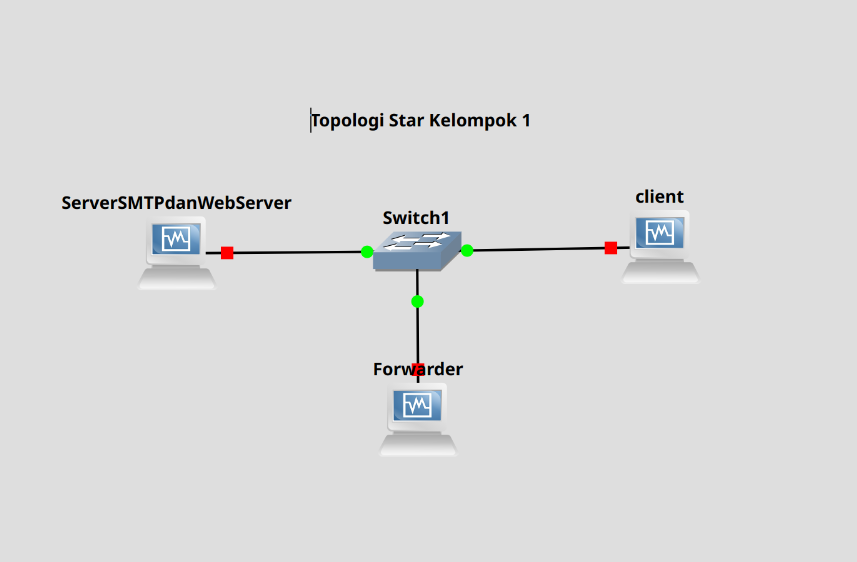
\includegraphics[width=12cm]{topologi.png}
    \caption{Topologi Star Sederhana}
    \label{fig:topologi}
  \end{figure}
\begin{adjustwidth}{1.4cm}{0cm}
\quad\quad Dalam proyek ini kami merancang dengan menggunakan topologi star sederhana. Di dalam topologi ini, kami menggunakan tiga virtual machine yaitu untuk client, forwarder, dan server. Dari masing masing virtual machine tersebut didalamnya berisi os linux yang saling terhubung satu sama lain dengan menggunakan jaringan lokal dengan ip class c. Untuk cara kerjanya sendiri yaitu, client digunakan untuk mengirimkan email ke fowarder menggunakan socket TCP, kemudian dari forwarder akan ditangkap dan diteruskan ke server dengan protokol SMTP.
\end{adjustwidth}
\subsection{Rincian Jaringan}

\begin{table}[h]
\centering
\begin{tabular}{|c|c|c|c|c|c|}
\hline
No. & Nama PC & IP Address & Subnet Mask & Operation System & Protokol \\ \hline
1   & Client  & 192.168.50.1 & 255.255.255.0 & Linux OS (Kali Linux) & TCP \\ \hline
2   & Forwarder & 192.168.50.2 & 255.255.255.0 & Linux OS (Debian 12) & TCP,SMTP \\ \hline
3   & Server  & 192.168.50.3 & 255.255.255.0 & Linux OS (Debian 12) & SMTP \\ \hline
\end{tabular}
\caption{Tabel Rincian Jaringan}
\end{table}
\pagebreak
\subsection{Konfigurasi PC Client}
\begin{enumerate}
  \item \textbf{Konfigurasi Jaringan} \\
  Untuk konfigurasi jaringan, digunakan metode `inet static` pada file `/etc/network/interfaces`. Berikut adalah contoh konfigurasi yang digunakan:
  \begin{figure}[h]
    \centering
    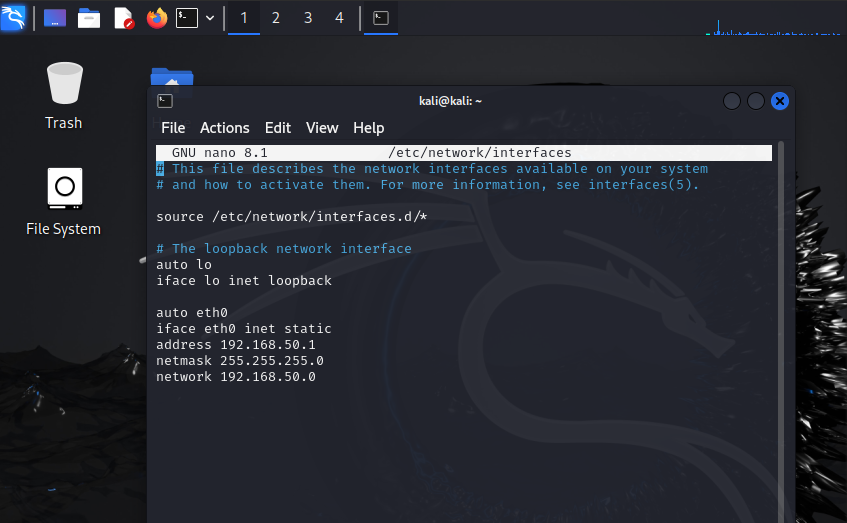
\includegraphics[width=12cm]{client.png}
    \caption{Konfigurasi IP Address}
  \end{figure}
  Konfigurasi tersebut mengatur alamat IP secara statis agar PC client terhubung dengan jaringan lokal menggunakan IP yang telah ditentukan yaitu 192.168.50.1
  \item \textbf{Cara Mengirimkan Email} \\
  Pada PC Client, untuk mengirimkan email ke forwarder, kami menggunakan socket TCP yang dikembangkan dengan bahasa pemrograman Rust. Untuk menjalankannya, kami menggunakan command cargo run, seperti yang dapat dilihat pada gambar di bawah ini.
    \begin{figure}[h]
    \centering
    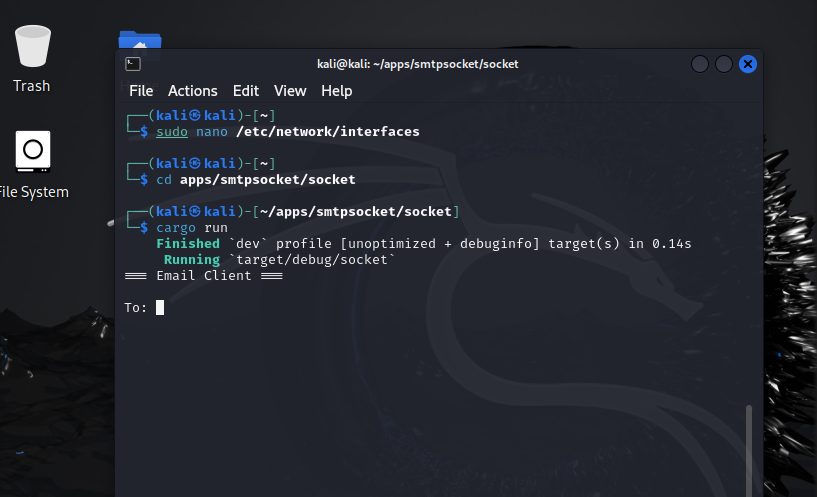
\includegraphics[width=12cm]{runclient.png}
    \caption{run program pc client }
  \end{figure}
  

  \item \textbf{Code Client}
\begin{minted}[linenos, breaklines]{rust}
use serde::Serialize;
use std::io::{self, Read, Write};
use std::net::TcpStream;

#[derive(Serialize)]
struct Email {
    sender: String,
    recipient: String,
    subject: String,
    body: String,
}

fn send_message(email: &str) {
    let server = "192.168.50.2:1239";

    match TcpStream::connect(server) {
        Ok(mut stream) => {
            println!("Succsessfully connected to forwarder {}", server);
            match stream.write_all(email.as_bytes()) {
                Ok(_) => {
                    println!("Try to sent email to forwarder");
                }
                Err(e) => {
                    println!("Failed to send email to forwarder {}", e);
                }
            }
            let mut response = String::new();
            match stream.read_to_string(&mut response) {
                Ok(_) => println!("Server response: {}", response),
                Err(e) => eprintln!("Failed to read server response: {}", e),
            }
        }
        Err(e) => {
            println!("Failed to connect to forwarder {}", e)
        }
    }
}

fn main() {
    let sender = "ketua@kelompoksatu.com";
    let mut recipient = String::new();
    let mut subject = String::new();
    let mut body = String::new();

    println!("=== Email Client ===\n");

    loop {
        print!("To: ");
        io::stdout().flush().unwrap();
        io::stdin().read_line(&mut recipient).unwrap();
        recipient = recipient.trim().to_string();
        print!("Subject: ");
        io::stdout().flush().unwrap();
        io::stdin().read_line(&mut subject).unwrap();
        subject = subject.trim().to_string();
        print!("body: ");
        io::stdout().flush().unwrap();
        io::stdin().read_line(&mut body).unwrap();
        body = body.trim().to_string();

        let email = Email {
            sender: sender.to_string(),
            recipient: recipient.clone(),
            subject: subject.clone(),
            body: body.clone(),
        };

        let email_json = serde_json::to_string(&email).unwrap();
        // println!("emaile: {}", email_json);
        send_message(&email_json);
        let mut choose = String::new();
        print!("LANJUT KIRIM LAGI ? y/n: ");
        io::stdout().flush().unwrap();
        io::stdin().read_line(&mut choose).unwrap();
        choose = choose.trim().to_string();
        if choose.eq_ignore_ascii_case("n") {
            break;
        }
        recipient.clear();
        body.clear();
    }
    println!("Seeee yooooouuuuuuuuuu");
}
\end{minted}

\end{enumerate}

\subsection{Konfigurasi PC forwarder}
\begin{enumerate}
  \item \textbf{Konfigurasi Jaringan} \\
  Pada pc forwarder juga dilakukan pengkonfigurasian ip static pada file `/etc/network/interfaces`, untuk lebih jelasnya bisa dilihat pada gammbar dibawah ini.
  \begin{figure}[h]
    \centering
    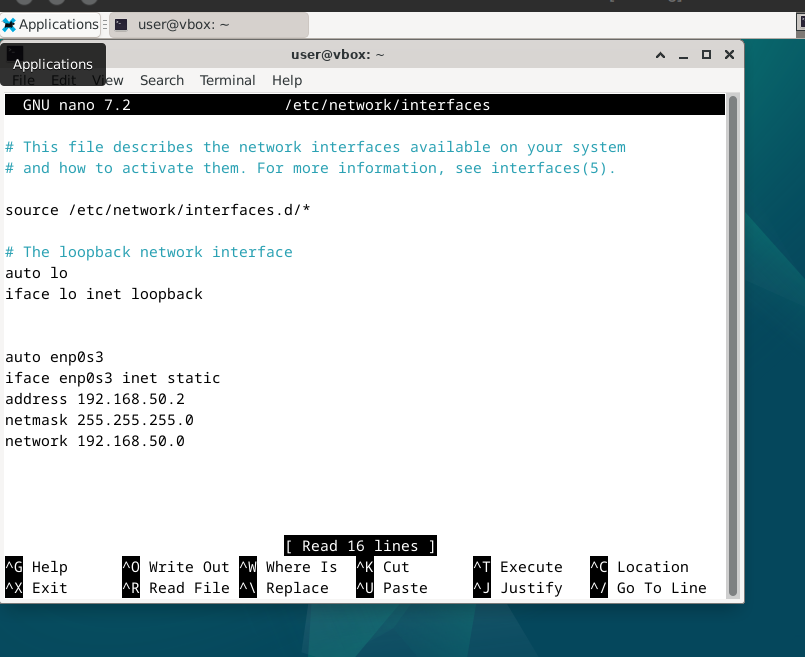
\includegraphics[width=12cm]{forwarder.png}
    \caption{Konfigurasi IP Address}
  \end{figure}
  Konfigurasi tersebut mengatur alamat IP secara statis agar PC forwarder ini dapat terhubung dengan jaringan lokal menggunakan IP yang telah ditentukan yaitu 192.168.50.2
  \item \textbf{Cara Menjalakan Forwarder} \\
    Pada pc forwarder kami menangkap data dari client yang akan diteruskan ke pc server. Untuk programnnya sendiri kami mengembangkannya dengan bahasa python sehingga untuk menjalankanya seperti gambar dibawah ini.
    \begin{figure}[h]
    \centering
    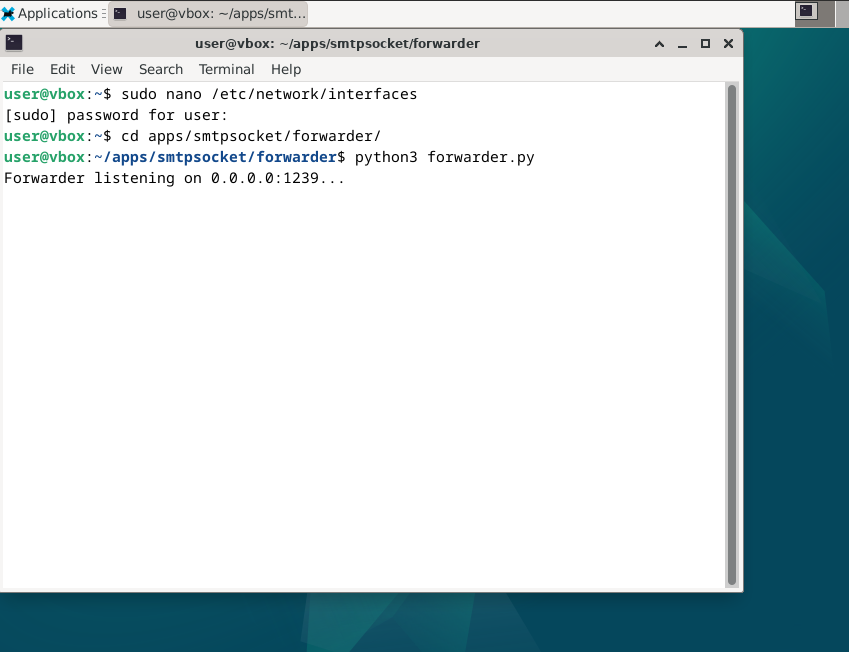
\includegraphics[width=12cm]{runforward.png}
    \caption{run program pc forwarder }
  \end{figure}
  
 \item \textbf{Code Forwarder}
 \begin{minted}[linenos, breaklines]{python}
import socket
import json
from threading import Thread
import smtplib
from email.mime.text import MIMEText
from email.mime.multipart import MIMEMultipart

def send_email_via_smtp(email_data):
    smtp_server = "192.168.50.3"  # IP dari PC3 (SMTP Server)
    smtp_port = 25            # Port yang sama seperti yang digunakan di server SMTP PC3

    try:
        # Membuat pesan email
        msg = MIMEMultipart()
        msg['From'] = email_data['sender']
        msg['To'] = email_data['recipient']
        msg['Subject'] = email_data['subject']
        msg.attach(MIMEText(email_data['body'], 'plain'))

        # Mengirim email melalui SMTP (PC3)
        with smtplib.SMTP(smtp_server, smtp_port) as server:
            server.sendmail(email_data['sender'], email_data['recipient'], msg.as_string())

        # print("Email successfully sent via SMTP.")
        return "Email successfully sent via SMTP."
    except Exception as e:
        # print(f"Error sending email via SMTP: {e}")
        error_message = f"Error sending email via SMTP error message: {e}"
        return error_message

def handle_client(client_socket):
    try:
        data = client_socket.recv(1024).decode()
        email_data = json.loads(data.replace("'", "\""))  # Parse the string as JSON
        print(f"Received email data: {email_data}")
        result = send_email_via_smtp(email_data)  # Kirim email via SMTP (ke PC3)
        print(f"iki lo hasil e {result.encode()}")
        client_socket.sendall(result.encode())

    except Exception as e:
        print(f"Error handling client: {e} {result}")
        client_socket.sendall(b"Failed to forward email".encode())
    finally:
        client_socket.close()

def start_forwarder(server_ip, server_port):
    with socket.socket(socket.AF_INET, socket.SOCK_STREAM) as server_socket:
        server_socket.bind((server_ip, server_port))
        server_socket.listen(5)
        print(f"Forwarder listening on {server_ip}:{server_port}...")
        while True:
            client_socket, addr = server_socket.accept()
            print(f"Connection established with {addr}")
            thread = Thread(target=handle_client, args=(client_socket,))
            thread.start()

if __name__ == "__main__":
    SERVER_IP = "0.0.0.0"
    SERVER_PORT = 1239
    start_forwarder(SERVER_IP, SERVER_PORT)
 \end{minted}
\end{enumerate}

\subsection{Konfigurasi PC Server}
\begin{enumerate}
  \item \textbf{Konfigurasi Jaringan} \\
  Pada pc server juga dilakukan pengkonfigurasian ip static pada file `/etc/network/interfaces`, untuk lebih jelasnya bisa dilihat pada gammbar dibawah ini.
  \begin{figure}[h]
    \centering
    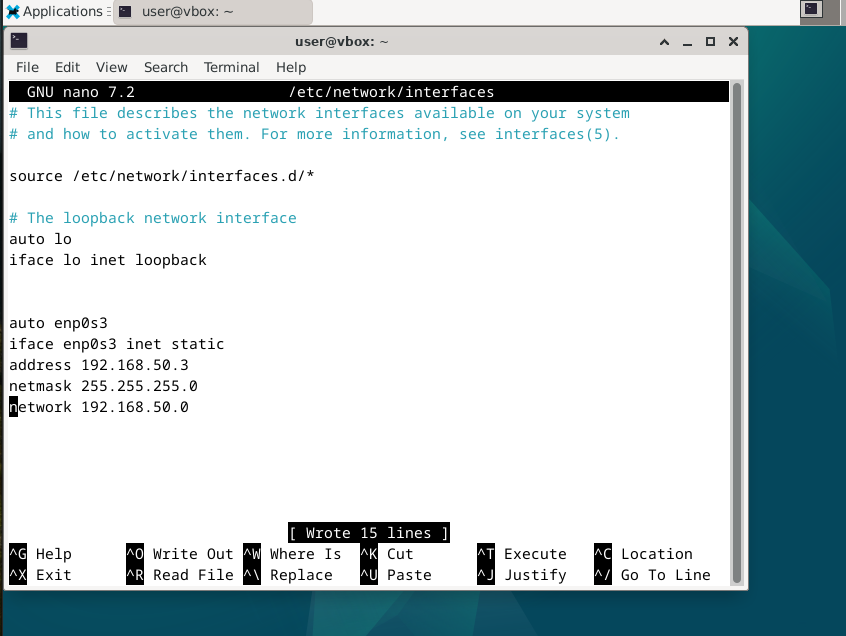
\includegraphics[width=12cm]{server.png}
    \caption{Konfigurasi IP Address}
  \end{figure}
  Konfigurasi tersebut mengatur alamat IP secara statis agar PC server ini dapat terhubung dengan jaringan lokal menggunakan IP yang telah ditentukan yaitu 192.168.50.3
  \item \textbf{Cara Menjalakan Server} \\
    Pada pc server kami menjalan dua program yaitu program SMTP server yang kami bangun dari bahasa rust dan web server yang kami bangun dari nodejs. Untuk perintah menjalankannya sendiri dapat dilihat pada gambar dibawah ini.
    \begin{figure}[h]
    \centering
    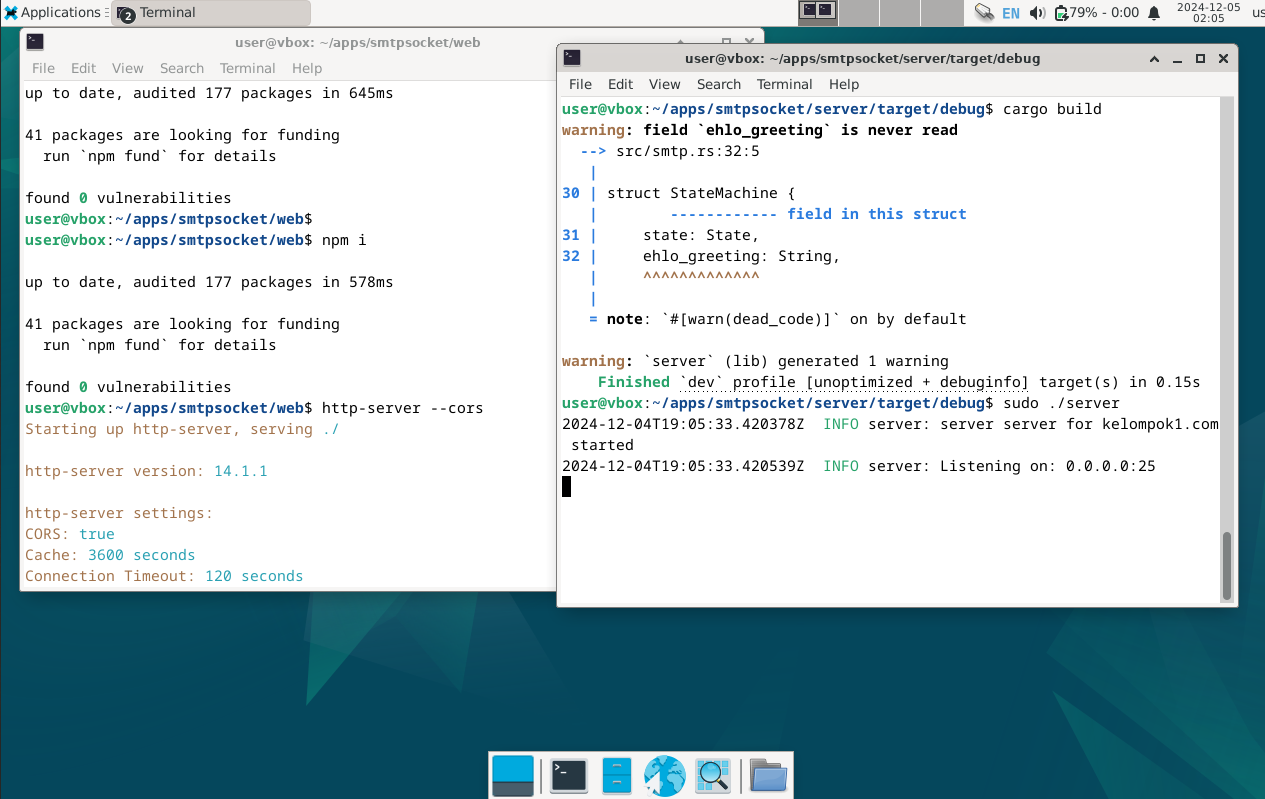
\includegraphics[width=12cm]{runserver.png}
    \caption{run program pc server }
  \end{figure}
\pagebreak

  \item \textbf{Code Server main.rs}
  \begin{minted}[linenos, breaklines]{rust}
  use anyhow::{Context, Result};
use tokio::net::TcpListener;

use std::env;

use server::smtp;

#[tokio::main]
async fn main() -> Result<()> {
    tracing_subscriber::fmt::init();

    let addr = env::args()
        .nth(1)
        .unwrap_or_else(|| "0.0.0.0:25".to_string());

    let domain = &env::args()
        .nth(2)
        .unwrap_or_else(|| "kelompok1.com".to_string());

    tracing::info!("server server for {domain} started");

    let listener = TcpListener::bind(&addr).await?;
    tracing::info!("Listening on: {}", addr);

    // Task for deleting old mail
    // periodically_clean_db(tokio::time::Duration::from_secs(3600));

    // Main loop: accept connections and spawn a task to handle them
    loop {
        let (stream, addr) = listener.accept().await?;
        tracing::info!("Accepted a connection from {}", addr);

        tokio::task::LocalSet::new()
            .run_until(async move {
                let smtp = smtp::Server::new(domain, stream).await?;
                tokio::time::timeout(std::time::Duration::from_secs(300), smtp.serve())
                    .await
                    .context("connection timed out")
            })
            .await
            .ok();
    }
}
  \end{minted}

  \item \textbf{Code Server smtp.rs}
   \begin{minted}[linenos, breaklines]{rust}
  use anyhow::{Context, Result};
use regex::Regex;
use serde::{Deserialize, Serialize};
use serde_json::{json, Value};
use std::fs::{self, OpenOptions};
use tokio::io::{AsyncReadExt, AsyncWriteExt};

#[derive(Clone, Debug, Default, PartialEq, Eq, Serialize, Deserialize)]
pub struct Mail {
    pub from: String,
    pub to: Vec<String>,
    pub data: String,
}

#[derive(Clone, Debug, PartialEq, Eq)]

enum State {
    Fresh,
    Greeted,
    ReceivingRcpt(Mail),
    ReceivingData(Mail),
    Received(Mail),
}

struct StateMachine {
    state: State,
    ehlo_greeting: String,
}

impl StateMachine {
    const OH_HAI: &'static [u8] = b"220 SMTP SERVER KELOMPOK 1 TRI B \n";
    const KTHXBYE: &'static [u8] = b"221 Bye\n";
    const HOLD_YOUR_HORSES: &'static [u8] = &[];

    pub fn new(domain: impl AsRef<str>) -> Self {
        let domain = domain.as_ref();
        let ehlo_greeting = format!("250-{domain} Hello {domain}\n250 AUTH PLAIN LOGIN\n");
        Self {
            state: State::Fresh,
            ehlo_greeting,
        }
    }

    pub fn handle_smtp(&mut self, raw_msg: &str) -> Result<&[u8]> {
        // let re_email = Regex::new(r"^[a-zA-Z0-9._%+-]+@[a-zA-Z0-9.-]+\.[a-zA-Z]{2,}$").unwrap();
        let re_email = Regex::new(r"^<([a-zA-Z0-9._%+-]+@[a-zA-Z0-9.-]+\.[a-zA-Z]{2,})>$").unwrap();

        const MAX_MSG_SIZE: usize = 10 * 1024 * 1024; // 10 MB

        tracing::trace!("Received {raw_msg} in state {:?}", self.state);
        let mut msg = raw_msg.split_whitespace();
        let command = msg.next().context("received empty command")?.to_lowercase();
        let state = std::mem::replace(&mut self.state, State::Fresh);

        match (command.as_str(), state) {
            ("ehlo", State::Fresh) => {
                tracing::trace!("Sending AUTH info and SIZE support");
                self.state = State::Greeted;
                Ok(b"250-Hello\r\n250-SIZE 10485760\r\n250 AUTH\r\n") // 10MB size limit
            }
            ("helo", State::Fresh) => {
                tracing::trace!("Received HELO");
                self.state = State::Greeted;
                Ok(b"250 Hello\r\n")
            }
            ("noop", _) | ("help", _) => {
                tracing::trace!("Got {command}");
                Ok(b"250 OK\r\n")
            }
            ("rset", _) => {
                tracing::trace!("Resetting state");
                self.state = State::Fresh;
                Ok(b"250 OK\r\n")
            }
            ("mail", State::Greeted) => {
                tracing::trace!("Receiving MAIL");
                let from = msg.next().context("received empty MAIL")?;
                let from = from
                    .strip_prefix("FROM:")
                    .context("received incorrect MAIL")?
                    .trim()
                    .to_string();
                if re_email.is_match(&from) {
                    tracing::debug!("Valid MAIL FROM: {from}");
                    self.state = State::ReceivingRcpt(Mail {
                        from: from.to_string(),
                        ..Default::default()
                    });
                    Ok(b"250 OK\r\n")
                } else {
                    tracing::warn!("Invalid MAIL FROM address: {from}");
                    Ok(b"501 Syntax: Invalid email address\r\n")
                }
            }
            ("rcpt", State::ReceivingRcpt(mut mail)) => {
                tracing::trace!("Receiving RCPT");
                let to = msg.next().context("received empty RCPT")?;
                let to = to
                    .strip_prefix("TO:")
                    .context("received incorrect RCPT")?
                    .trim();
                if re_email.is_match(to) {
                    tracing::debug!("Valid RCPT TO: {to}");
                    mail.to.push(to.to_lowercase());
                    self.state = State::ReceivingRcpt(mail);
                    Ok(b"250 OK\r\n")
                } else {
                    tracing::warn!("Invalid RCPT TO address: {to}");
                    Ok(b"501 Syntax: Invalid recipient address\r\n")
                }
            }
            ("data", State::ReceivingRcpt(mail)) => {
                if mail.to.is_empty() {
                    tracing::warn!("DATA command received without RCPT");
                    Ok(b"503 Error: RCPT TO command must precede DATA\r\n")
                } else {
                    tracing::trace!("Ready to receive DATA");
                    self.state = State::ReceivingData(mail);
                    Ok(b"354 Start mail input; end with <CR><LF>.<CR><LF>\r\n")
                }
            }
            ("quit", State::ReceivingData(mail)) => {
                self.state = State::Received(mail);
                Ok(StateMachine::KTHXBYE)
            }
            (_, State::ReceivingData(mut mail)) => {
                tracing::trace!("Appending data");
                if raw_msg.ends_with("\r\n.\r\n") {
                    let trimmed_data = raw_msg.trim_end_matches("\r\n.\r\n");
                    mail.data.push_str(trimmed_data);
                    if mail.data.len() > MAX_MSG_SIZE {
                        tracing::warn!("Message size exceeds limit");
                        Ok(b"552 Error: Message size exceeds maximum size\r\n")
                    } else {
                        tracing::trace!(
                            "Email received: FROM: {} TO: {:?} DATA: {}",
                            mail.from,
                            mail.to,
                            mail.data
                        );
                        mail.data += raw_msg;
                        self.state = State::ReceivingData(mail);
                        Ok(b"250 OK\r\n")
                    }
                } else {
                    mail.data.push_str(raw_msg);
                    self.state = State::ReceivingData(mail);
                    Ok(b"250 Continue\r\n")
                }
            }
            _ => {
                tracing::warn!("Unexpected message: {raw_msg}");
                Ok(b"500 Syntax error, command unrecognized\r\n")
            }
        }
    }

}

pub struct Server {
    stream: tokio::net::TcpStream,
    state_machine: StateMachine,
}

impl Server {
    pub async fn new(domain: impl AsRef<str>, stream: tokio::net::TcpStream) -> Result<Self> {
        Ok(Self {
            stream,
            state_machine: StateMachine::new(domain),
        })
    }

    pub async fn serve(mut self) -> Result<()> {
        self.greet().await?;

        let mut buf = vec![0; 1024 * 1024];
        loop {
            let n = self.stream.read(&mut buf).await?;

            if n == 0 {
                self.state_machine.handle_smtp("quit").ok();
                break;
            }
            let msg = std::str::from_utf8(&buf[0..n])?;
            let response = self.state_machine.handle_smtp(msg)?;
            if response != StateMachine::HOLD_YOUR_HORSES {
                self.stream.write_all(response).await?;
            }
            if response == StateMachine::KTHXBYE {
                break;
            }
        }

        match self.state_machine.state {
            State::Received(ref mail) => {
                self.save_email_to_json(mail).await?;
            }
            State::ReceivingData(ref mail) => {
                self.save_email_to_json(mail).await?;
            }
            _ => {}
        }
        Ok(())
    }

    async fn save_email_to_json(&self, mail: &Mail) -> Result<()> {
        let file_path = "received_email.json";
        let email_entry = json!({
            "sender": mail.from,
            "recipient": mail.to,
            "subject": self.extract_subject(&mail.data)?,
            "body": self.extract_body(&mail.data)?,
        });

        let mut emails: Vec<Value> = if let Ok(existing_content) = fs::read_to_string(file_path) {
            serde_json::from_str(&existing_content)?
        } else {
            Vec::new()
        };

        emails.push(email_entry);

        let file = OpenOptions::new()
            .write(true)
            .create(true)
            .truncate(true)
            .open(file_path)?;
        serde_json::to_writer_pretty(file, &emails)?;
        println!("Email saved to {}", file_path);

        Ok(())
    }

    fn extract_subject(&self, data: &str) -> Result<String> {
        for line in data.lines() {
            if line.to_lowercase().starts_with("subject:") {
                return Ok(line[8..].trim().to_string());
            }
        }
        Ok("No Subject".to_string())
    }

    fn extract_body(&self, data: &str) -> Result<String> {
        if let Some(boundary_start) = data.find("--===") {
            let body_start = data[boundary_start..]
                .find("\r\n\r\n")
                .map(|pos| boundary_start + pos + 4)
                .unwrap_or(data.len());
            let body_end = data[body_start..]
                .find("\r\n--===")
                .map(|pos| body_start + pos)
                .unwrap_or(data.len());
            return Ok(data[body_start..body_end].trim().to_string());
        }

        if let Some(headers_end) = data.find("\r\n\r\n") {
            return Ok(data[headers_end + 4..].trim().to_string());
        }

        Ok("No Body Found".to_string())
    }

    async fn greet(&mut self) -> Result<()> {
        self.stream
            .write_all(StateMachine::OH_HAI)
            .await
            .map_err(|e| e.into())
    }
}

#[cfg(test)]
mod tests {
    use super::*;

    #[test]
    fn test_regular_flow() {
        let mut sm = StateMachine::new("dummy");
        sm.handle_smtp("HELO localhost").unwrap();
        sm.handle_smtp("MAIL FROM: <local@example.com>").unwrap();
        sm.handle_smtp("RCPT TO: <a@localhost.com>").unwrap();
        sm.handle_smtp("RCPT TO: <b@localhost.com>").unwrap();
        sm.handle_smtp("DATA hello world\n").unwrap();
        sm.handle_smtp("QUIT").unwrap();
    }

    #[test]
    fn test_no_greeting() {
        let mut sm = StateMachine::new("dummy");
        for command in [
            "MAIL FROM: <local@example.com>",
            "RCPT TO: <local@example.com>",
            "DATA hey",
            "GARBAGE",
        ] {
            assert!(sm.handle_smtp(command).is_err());
        }
    }
}

#[test]
fn test_no_greeting() {
    let re_email = Regex::new(r"^<([a-zA-Z0-9._%+-]+@[a-zA-Z0-9.-]+\.[a-zA-Z]{2,})>$").unwrap();
    let email = "<ketua@kelompoksatu.com>";
    println!("Valid email: {}", re_email.is_match(email));
}

   \end{minted}
\end{enumerate}
\pagebreak

\section{\centering\\SIMULASI DAN HASIL TEST-BED}

\subsection{Pengujian Antar PC}
\begin{enumerate}
\item Pada saat client mengirim, forwarder dan server mati
\begin{figure}[!ht]
    \centering
    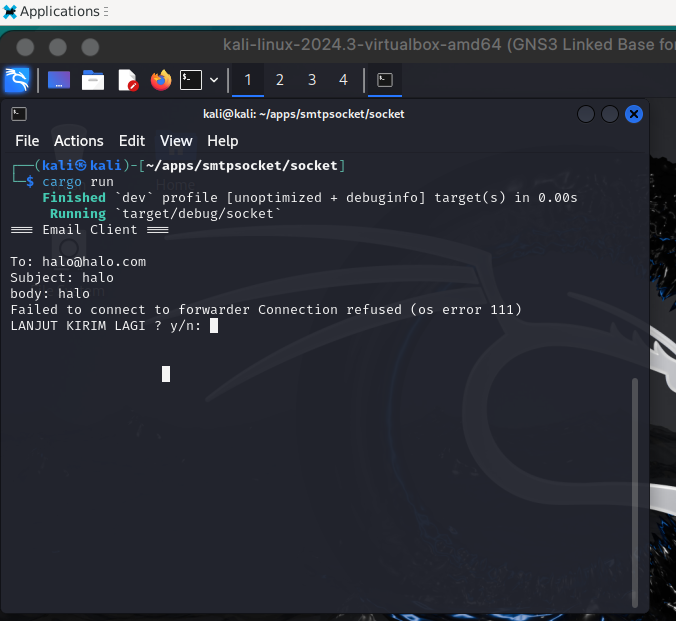
\includegraphics[width=10cm]{bab 3/tes1.png}
    \caption{Client hidup, forwarder dan server mati}
\end{figure}
\item Pada saat PC client dan forwarder hidup, pc Server mati
\begin{figure}[!ht]
    \centering
    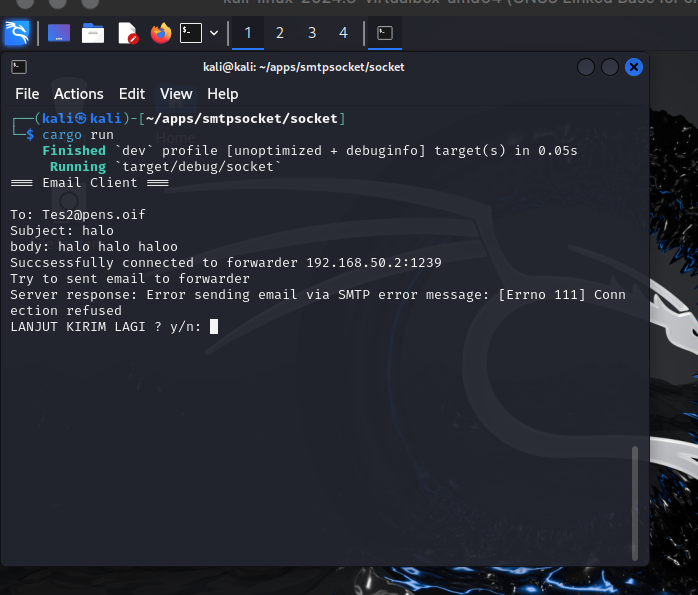
\includegraphics[width=10cm]{bab 3/tes2.png}
    \caption{Client forwarder hidup dan server mati}
\end{figure}
\pagebreak
\item Pada saat semua pc hidup 
 \begin{figure}[h]
    \centering
    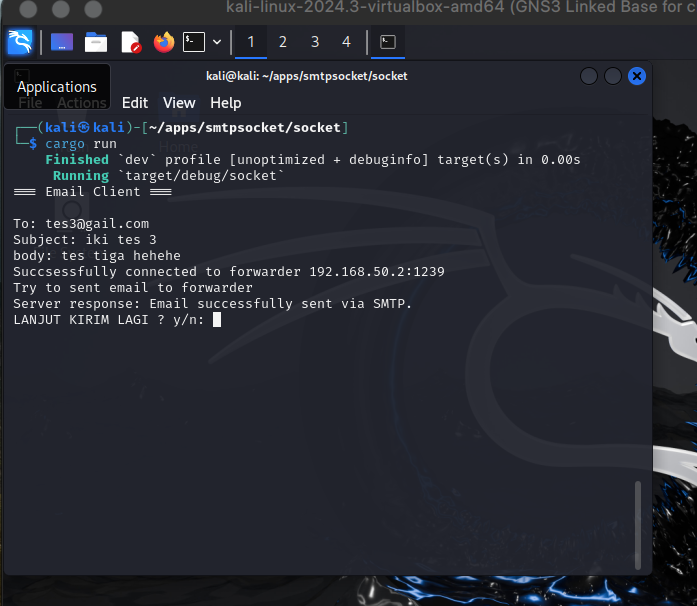
\includegraphics[width=10cm]{bab 3/tes3.png}
    \caption{semua pc hidup}
  \end{figure}
  \end{enumerate}
\subsection{Hasil pada webserver ketika berhasil}
 \begin{figure}[h]
    \centering
    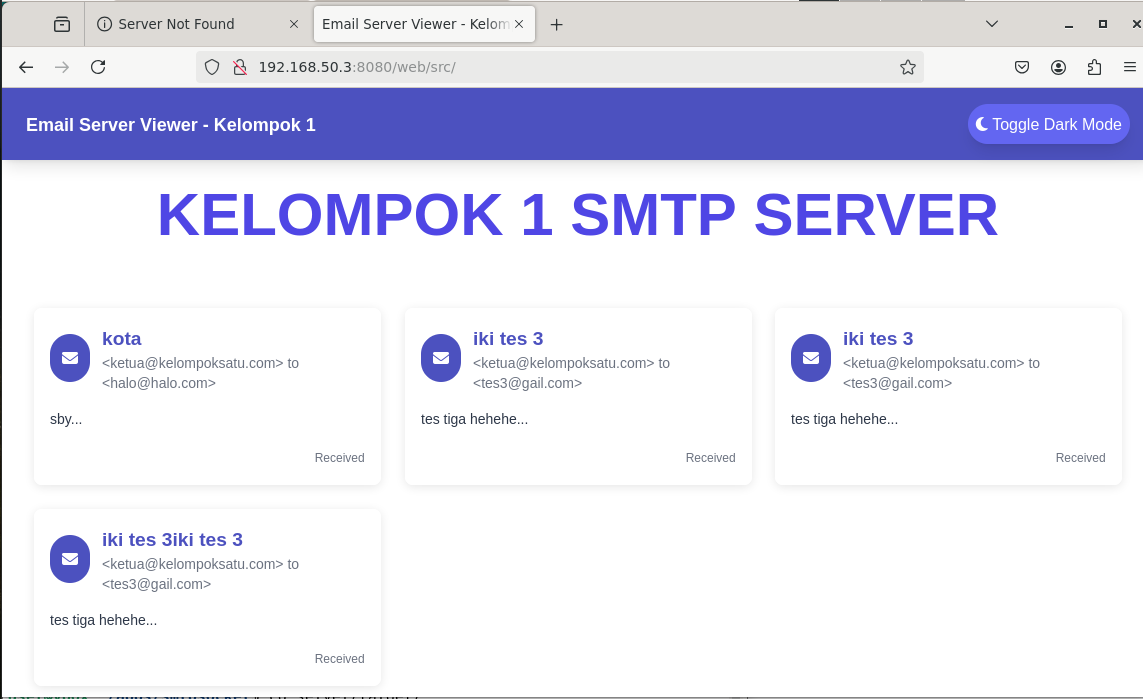
\includegraphics[width=10cm]{bab 3/tes4.png}
    \caption{Hasil tampilan web server}
  \end{figure}
\clearpage
\subsection{Test Menggunakan telnet dari pc client ke SMTP server}
 \begin{figure}[h]
    \centering
    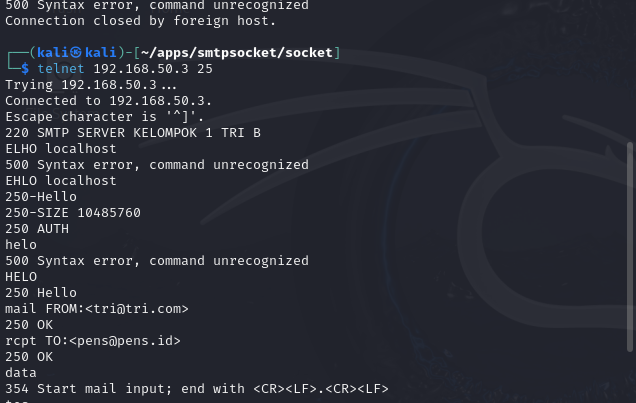
\includegraphics[width=10cm]{bab 3/tes5.png}
    \caption{test dengan telnet}
  \end{figure}

\subsection{Hasil Capture dari Wireshark}
\begin{enumerate}
\item Data yang dikirim
\begin{figure}[!ht]
    \centering
    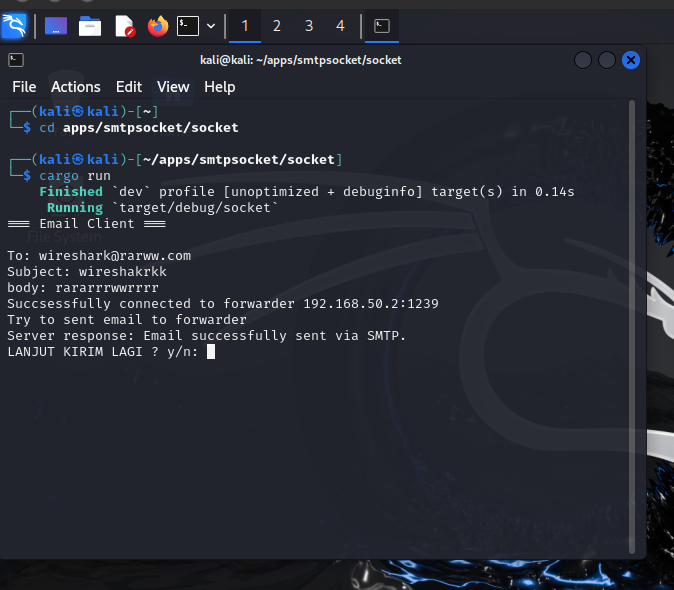
\includegraphics[width=10cm]{bab 3/data.png}
    \caption{data yang dikirim}
\end{figure}
\clearpage
\item Socket TCP
\begin{figure}[!ht]
    \centering
    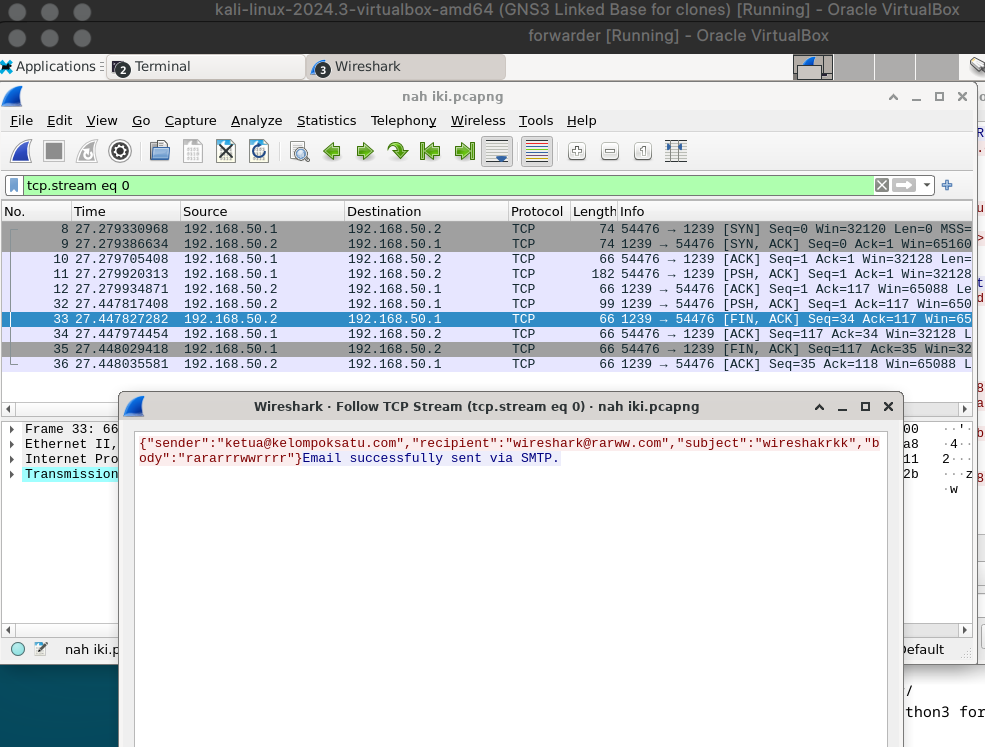
\includegraphics[width=10cm]{bab 3/tcp0.png}
    \caption{Socket TCP}
\end{figure}
\item SMTP  
 \begin{figure}[h]
    \centering
    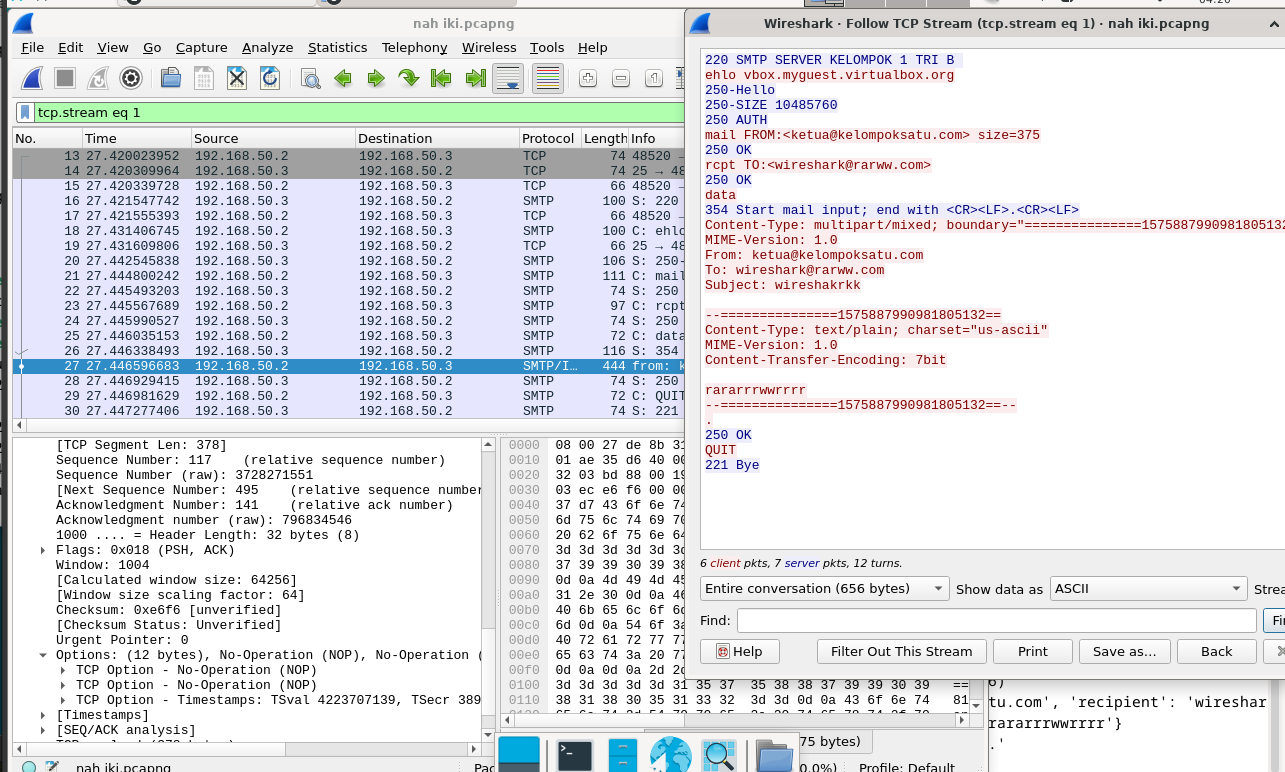
\includegraphics[width=10cm]{bab 3/tcp1.png}
    \caption{SMTP}
  \end{figure}
\end{enumerate}
\pagebreak
\section{\centering\\ANALISA}
\quad\quad Pada hasil percobaan yang telah dilakukan didapatkan analisa yaitu sistem ini dirancang untuk mengirimkan pesan melalui email dan menampilkannya di halaman web secara dengan menggunkan nodejs. Sistem yang dibangun terdiri dari tiga komponen utama, yaitu client, server forwarder, dan server email. Ketiganya berkomunikasi menggunakan protokol TCP untuk memastikan stabilitas dan efisiensi dalam pengiriman pesan.

Proses pengiriman dimulai ketika klien mengirimkan data email ke server forwarder melalui koneksi socket TCP. Forwarder berfungsi sebagai jembatan antara klien dan server SMTP, bertugas untuk menerima pesan dari klien, memvalidasinya, dan meneruskannya ke server SMTP. Selain itu, forwarder bertanggung jawab untuk memberikan respons kepada klien, baik ketika pesan berhasil diterima maupun ketika terjadi kegagalan. Respons ini dikirim dalam bentuk status kode, memungkinkan klien mengetahui hasil dari pengiriman pesan.

Setelah menerima data dari klien, forwarder meneruskannya ke server SMTP menggunakan protokol SMTP. Pada proyek ini, server SMTP dibangun menggunakan bahasa pemrograman Rust, dengan mengacu pada spesifikasi dalam RFC 5321 sebagai pedoman utama. RFC 5321 menyediakan standar dan aturan rinci untuk menangani perintah-perintah SMTP seperti HELO/EHLO, MAIL FROM, RCPT TO, dan DATA, serta untuk memastikan pengiriman pesan yang sesuai dengan protokol.

Namun, terdapat beberapa tantangan dalam membangun server SMTP ini. Salah satu tantangan utama adalah memastikan bahwa server SMTP dapat menangani semua perintah, status, dan respons sesuai dengan spesifikasi RFC 5321. Implementasi harus mencakup kemampuan untuk memproses berbagai status kode seperti 250 OK, 501 Syntax: Invalid email address, dan kode lainnya, yang kemudian dikirim kembali ke forwarder. Forwarder bertugas untuk meneruskan status ini ke klien sehingga klien dapat menerima umpan balik secara real-time. Selain itu juga Dari server SMTP Ini apabila berhasil maka menyimpan data dari client untuk ditampilkan ke browser dengan menggunakan web server dalam hal ini kami menggunkan node js.
\begin{adjustwidth}{1.4cm}{0cm}
\quad\quad 
\end{adjustwidth}

\pagebreak
\section{\centering\\ KESIMPULAN}
\subsection{Kesimpulan}
\begin{adjustwidth}{1.4cm}{0cm}
\quad\quad Kesimpulan yang bisa kita ambil yaitu, sistem yang berhasil di rancang dan di implementasikan sistem pengiriman pesan melalui email dengan mengintegerasikan tiga komponen pendukung, yaitu client, forwarder, dan server email. Komunikasi antar satu sama lain menggunakan protokol TCP untuk memastikan efiesiensi dan stabil nya komunikasi tersebut. 
Untuk server forwarder berperan sebagai penghubung antar client dan server SMTP, bertugas untuk memverifikasi,  meneruskan pesan, serta memberikan respon status berhasilnya dikirim ke client. Server SMTP yang di operasikan menggunakan bahasa Rust telah di implementasikan sesuai standar RFC 5321, untuk menangani perintah-perintah protokol SMTP serta status dan respons nya dengan cepat.
Selain untuk pengiriman email, sistem ini juga memungkinkan penyimpanan data email di server yang di terima dari client melalui web server yang  berbasis Node.js. Walaupun terdapat tantangan teknis dalam memastikan kesesuaian implementasi dengan spesifikasi protokol SMTP, sistem ini telah mampu untuk memberikan umpan balik secara real time kepada client dan mendukung pengiriman pesan yang efisien.
\end{adjustwidth}

\end{document}